\def\advent@xx@i{
  It is possible to write 325 different numbers using the digits 1, 2, 3, 4, and 5 at most once each (and using no other digits).
  How many of these numbers are odd?
}

\def\advent@xx@ii{
  Carol draws a square with area 62.
  She then draws the smallest possible circle that this square is contained inside.
  Next, she draws the smallest possible square that her circle is contained inside.
  What is the area of her second square?
}

\def\advent@xx@iii{
  Put the digits 1 to 9 (using each digit exactly once) in the boxes so that the sums are correct.
  The sums should be read left to right and top to bottom ignoring the usual order of operations.
  For example, $4 + 3 \times 2$ is 14, not 10. Today's number is the largest number you can make with the digits in the red boxes.

  \grid@advent@xx@iii{}{}{}{}{}{}{}{}{}
}

\def\advent@xx@iv{
  Today's number is a three digit number which is equal to the sum of the cubes of its digits.
  One less than today's number also has this property.
}

\def\advent@xx@v{
  Carol rolled a large handful of six-sided dice. The total of all the numbers Carol got was 521.
  After some calculating, Carol worked out that the probability that of her total being 521 was the same as the probability that her total being 200.
  How many dice did Carol roll?
}

\def\advent@xx@vi{
  There are 12 ways of placing 2 tokens on a $2 \times 4$ grid so that no two tokens are next to each other horizontally, vertically or diagonally:
  \begin{center}
    \begin{tikzpicture}
      % Draw all the grids
      \foreach \gi in {0,1}{
          \foreach \gj in {0,...,5}{
              \foreach \i in {0,1}{
                  \foreach \j in {0,...,3}{
                      \gridbox{5*\gj + \j}{3*\gi + \i}{}
                    }
                }
            }
        }

      % Place token circles
      \gridcirc{0}{4}
      \gridcirc{2}{4}
      \gridcirc{5}{4}
      \gridcirc{8}{4}
      \gridcirc{10}{4}
      \gridcirc{12}{3}
      \gridcirc{15}{4}
      \gridcirc{18}{3}
      \gridcirc{21}{4}
      \gridcirc{23}{4}
      \gridcirc{26}{4}
      \gridcirc{28}{3}
      \gridcirc{0}{0}
      \gridcirc{2}{1}
      \gridcirc{5}{0}
      \gridcirc{8}{1}
      \gridcirc{11}{0}
      \gridcirc{13}{1}
      \gridcirc{15}{0}
      \gridcirc{17}{0}
      \gridcirc{20}{0}
      \gridcirc{23}{0}
      \gridcirc{26}{0}
      \gridcirc{28}{0}
    \end{tikzpicture}
  \end{center}

  Today's number is the number of ways of placing 5 tokens on a $2 \times 10$ grid so that no two tokens are next to each other horizontally, vertically or diagonally.
}

\newcommand\domino[4]{
  \gridbox{#1}{#2}{#3}
  \gridbox{#1 + 1}{#2}{#4}
}
\def\advent@xx@vii{
  There are 15 dominoes that can be made using the numbers 0 to 4 (inclusive):
  \begin{center}
    \begin{tikzpicture}
      \newcounter{dn}
      \newcounter{row}
      \foreach \gi in {0,...,4}{
          \foreach \gj in {\gi,...,4}{
              \domino{3*\value{dn}}{-2*\value{row}}{\gi}{\gj}
              \stepcounter{dn}
              \ifnum\value{dn} = 9
              \setcounter{dn}{0}
              \stepcounter{row}
              \fi
            }
        }
    \end{tikzpicture}
  \end{center}

  The sum of all the numbers on all these dominoes is 60.

  Today's number is the sum of all the numbers on all the dominoes that can be made using the numbers 5 to 10 (inclusive).
}

\def\advent@xx@viii{
  The residents of Octingham have 8 fingers.
  Instead of counting in base ten, they count in base eight: the digits of their numbers represent ones, eights, sixty-fours, two-hundred-and-fifty-sixes, etc instead of ones, tens, hundreds, thousands, etc.

  For example, a residents of Octingham would say 12, 22 and 52 instead of our usual numbers 10, 18 and 42.

  Today's number is what a resident of Octingham would call 11 squared (where the 11 is also written using the Octingham number system).
}

\def\advent@xx@ix{
  Put the digits 1 to 9 (using each digit exactly once) in the boxes so that the sums are correct.
  The sums should be read left to right and top to bottom ignoring the usual order of operations.
  For example, $4 + 3 \times 2$ is 14, not 10.
  Today's number is the product of the numbers in the red boxes.

  \grid@advent@xx@ix{}{}{}{}{}{}{}{}{}
}

\def\advent@xx@x{
  Today's number is the smallest multiple of 24 whose digits add up to 24.
}

\def\advent@xx@xi{
  Noel has a large pile of cards.
  Half of them are red, the other half are black.
  Noel splits the cards into two piles: pile A and pile B.

  Two thirds of the cards in pile A are red.
  Noel then moves 108 red cards from pile A to pile B.
  After this move, two thirds of the cards in pile B are red.

  How many cards did Noel start with?
}

\def\advent@xx@xii{
  The diagram below shows a large black square.
  Inside this square, two red squares have been drawn.
  (The sides of the red squares are parallel to the sides of the black square; each red square shares a vertex with the black square; and the two red squares share a vertex.)
  A blue quadrilateral has then been drawn with vertices at two corners of the black square and the centers of the red squares.

  The area of the blue quadrilateral is 167. What is the area of the black square?

  \begin{center}
    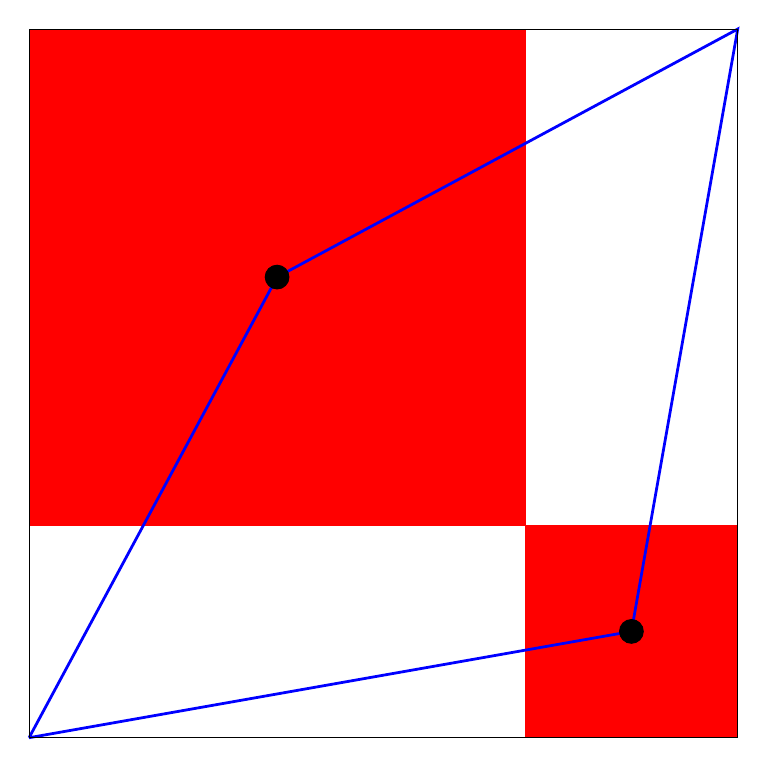
\begin{tikzpicture}
      \def\bss{9}
      \def\mpt{0.7}
      \coordinate (A) at (\mpt * \bss / 2, -\mpt * \bss / 2);
      \coordinate (B) at (\mpt * \bss /2 + \bss/2, -\mpt * \bss /2 - \bss/2);
      \filldraw[draw=black, color=red] (0, 0) rectangle (\mpt * \bss, -\mpt * \bss);
      \filldraw[draw=black, color=red] (\mpt * \bss, -\mpt * \bss) rectangle (\bss, -\bss);
      \draw[line width=1, color=blue] (0,-\bss) -- (A) -- (\bss, 0) -- (B) -- (0, -\bss);
      \draw[fill=black] (A) circle (0.15);
      \draw[fill=black] (B) circle (0.15);
      \draw (0,0) rectangle (\bss,-\bss);
    \end{tikzpicture}
  \end{center}
}

\def\advent@xx@xiii{
  There are 6 ways to split the sequence of the numbers 1 to 5 into three shorter sequences:
  \begin{itemize}
    \item 1 and 2 and 3, 4, 5
    \item 1 and 2, 3 and 4, 5
    \item 1 and 2, 3, 4 and 5
    \item 1, 2 and 3 and 4, 5
    \item 1, 2 and 3, 4 and 5
    \item 1, 2, 3 and 4 and 5
  \end{itemize}

  Today's number if the number of ways to split the sequence of the numbers 1 to 10 into five shorter sequences.
}

\def\advent@xx@xiv{
  The numbers 33, 404 and 311 contain duplicate digits. The numbers 120, 15 and 312 do not.

  How many numbers between 10 and 999 (inclusive) contain no duplicate digits?
}

\def\advent@xx@xv{
  When talking to someone about this Advent calendar, you told them that the combination of XMAS and MATHS is GREAT.
  They were American, so asked you if the combination of XMAS and MATH is great; you said SURE.
  You asked them their name; they said SAM.

  Each of the letters E, X, M, A, T, H, S, R, U, and G stands for a different digit 0 to 9.
  The following sums are correct:
  \begin{center}
    \begin{multicols}{2}
      \begin{tabular}{cccccc}
            &   & X & M & A & S \\
        $+$ & M & A & T & H & S \\
        \hline
            & G & R & E & A & T
      \end{tabular}

      \begin{tabular}{ccccc}
            & X & M & A & S \\
        $+$ & M & A & T & H \\
        \hline
            & S & U & R & E
      \end{tabular}
    \end{multicols}
  \end{center}

  Today's number is SAM. To help you get started, the letter T represents 4.
}

\def\advent@xx@xvi{
  Solve the crossnumber to find today's number.
  No number starts with 0.
  \begin{multicols}{2}
    \crossnumstd{}{}{}{}{}{}{}{}{}

    \vfill\null
    \columnbreak

    \begin{center}
      \textbf{Across}

      \begin{tabular}{clc}
        \textbf{1} & 3 more than a multiple of 110.  & (\textbf{3}) \\
        \textbf{4} & Today's number.                 & (\textbf{3}) \\
        \textbf{5} & 30 more than a multiple of 101. & (\textbf{3})
      \end{tabular}

      \textbf{Down}

      \begin{tabular}{clc}
        \textbf{1} & 37 times the sum of 1A's digits. & (\textbf{3}) \\
        \textbf{2} & 3 times a factor of 5A.          & (\textbf{3}) \\
        \textbf{3} & 3 less than a multiple of 112.   & (\textbf{3})
      \end{tabular}
    \end{center}
  \end{multicols}
}

\def\advent@xx@xvii{
  Put the digits 1 to 9 (using each digit exactly once) in the boxes so that the sums and product are correct.
  Today's number is the product of the numbers in the red boxes.

  \grid@advent@xx@xvii{}{}{}{}{}{}{}{}{}
}

\def\advent@xx@xviii{
  The expansion of $(x + y + z)^3$ is
  \gath{
    x^3 + y^3 + z^3 + 3x^2y + 3x^2z + 3xy^2 + 3y^2z + 3xz^2 + 3yz^2 + 6xyz \, .
  }
  This has 10 terms.

  Today's number is the number of terms in the expansion of $(x+y+z)^{26}$.
}

\def\advent@xx@xix{
  The diagram below shows a triangle.
  Two of the sides of the triangle have been split into three pieces, with lines drawn from the opposite vertex.
  In total, the diagram now contains 27 triangles of any size.

  Another triangle has two of its sides split into eight pieces, with lines drawn from the opposite vertex.
  How many triangles (of any size) would this create?

  \begin{center}
    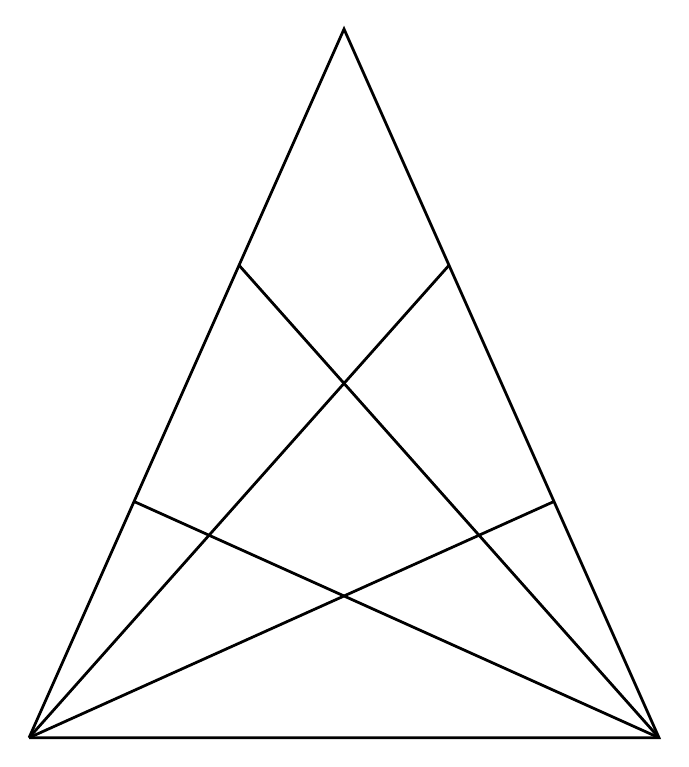
\begin{tikzpicture}[scale=2]
      % Draw triangle
      \def\ht{4.5}
      \def\wd{4}
      \draw[line width=1] (0,0) -- (\wd / 2, \ht) -- (\wd, 0) -- (0, 0);

      % Other lines
      \draw[line width=1] (\wd, 0) -- (\wd / 6, \ht / 3);
      \draw[line width=1] (\wd, 0) -- (\wd / 3, 2*\ht / 3);
      \draw[line width=1] (0, 0) -- (2*\wd / 3, 2*\ht / 3);
      \draw[line width=1] (0, 0) -- (5*\wd / 6, \ht / 3);
    \end{tikzpicture}
  \end{center}
}

\def\advent@xx@xx{
  18 can be written as the sum of 3 consecutive (strictly) positive integers: 5 + 6 + 7.

  18 can also be written as the sum of 4 consecutive (strictly) positive integers: 3 + 4 + 5 + 6.

  18 is in fact the smallest number that can be written as the sum of both 3 and 4 consecutive (strictly) positive integers.

  Today's number is the smallest number that can be written as the sum of both 12 and 13 consecutive (strictly) positive integers.
}

\def\advent@xx@xxi{
  There are 3 ways to order the numbers 1 to 3 so that no number immediately follows the number one less that itself:
  \begin{itemize}
    \item 3, 2, 1
    \item 1, 3, 2
    \item 2, 1, 3
  \end{itemize}
  Today's number is the number of ways to order the numbers 1 to 6 so that no number immediately follows the number one less that itself.
}

\def\advent@xx@xxii{
  Put the digits 1 to 9 (using each digit exactly once) in the boxes so that the sums are correct.
  The sums should be read left to right and top to bottom ignoring the usual order of operations.
  For example, $4 + 3 \times 2$ is 14, not 10.
  Today's number is the largest number you can make with the digits in the red boxes.

  \grid@advent@xx@xxii{}{}{}{}{}{}{}{}{}
}

\def\advent@xx@xxiii{
  198 is the smallest number that is equal to 11 times the sum of its digits.

  Today's number is the smallest number that is equal to 48 times the sum of its digits.
}

\def\advent@xx@xxiv{
  There are six ways to put two tokens in a 3 by 3 grid so that the diagonal from the top left to the bottom right is a line of symmetry:
  \begin{center}
    \begin{tikzpicture}
      % Draw all the grids
      \foreach \gj in {0,...,5}{
          \foreach \i in {0,...,2}{
              \foreach \j in {0,...,2}{
                  \gridbox{4*\gj + \j}{\i}{}
                }
            }
        }

      % Place token circles
      \gridcirc{0}{2}
      \gridcirc{1}{1}
      \gridcirc{5}{2}
      \gridcirc{4}{1}
      \gridcirc{8}{2}
      \gridcirc{10}{0}
      \gridcirc{14}{2}
      \gridcirc{12}{0}
      \gridcirc{17}{1}
      \gridcirc{18}{0}
      \gridcirc{22}{1}
      \gridcirc{21}{0}
    \end{tikzpicture}
  \end{center}

  Today's number is the number of ways of placing two tokens in a 29 by 29 grid so that the diagonal from the top left to the bottom right is a line of symmetry.
}

\def\card@xx@i{
  How many odd numbers can you make (by writing digits next to each other, so 13, 1253, and 457 all count) using the digits 1, 2, 3, 4, 5, and 7 each at most once (and no other digits)?
}

\def\card@xx@ii{
  Carol made a book by stacking 40300 pieces of paper, folding the stack in half, then writing the numbers 1 to 161200 on the pages.
  She then pulled out one piece of paper and added up the four numbers written on it.
  What is the largest number she could have reached?
}

\def\card@xx@iii{
  What is the sum of all the odd numbers between 0 and 130376?
}

\def\card@xx@iv{
  There are three cards with integers written on them.
  The pairs of cards add to 31, 35 and 36. What is the sum of all three cards?
}

\def\card@xx@v{
  What is the volume of the smallest cuboid that a square-based pyramid with volume 1337 can fit inside?
}

\def\card@xx@vi{
  What is the lowest common multiple of 305 and 671?
}

\def\card@xx@vii{
  Holly rolled a huge pile of dice and added up all the top faces to get 6136.
  She realized that the probability of getting 6136 was the same as getting 9999.
  How many dice did she roll?
}

\def\card@xx@viii{
  How many squares (of any size) are there in a $14 \times 16$ grid of squares?
}

\def\card@xx@ix{
  Ivy picked a number, removed a digit, then added her two numbers to get 155667. What was her original number?
}
